% =====================================================================
% Why doesn't the model diverge?
% The Gaussian null regime and the case for structural divergence
%
% Build:  pdflatex -interaction=nonstopmode structural_divergence_talk.tex
% (run twice; figures resolve via \graphicspath to ../figures/)
% =====================================================================
\documentclass[aspectratio=169,11pt]{beamer}

\usetheme{default}
\usefonttheme{professionalfonts}
\setbeamertemplate{navigation symbols}{}
\setbeamertemplate{footline}[frame number]

\usepackage{amsmath,amssymb,bm}
\usepackage{graphicx}
\usepackage{tikz}
\usetikzlibrary{arrows.meta,positioning,fit,backgrounds,calc,decorations.pathmorphing,decorations.pathreplacing}
\usepackage{pgfplots}
\pgfplotsset{compat=1.17}

\graphicspath{{../figures/}}

% ---------------------------------------------------------------- palette
\definecolor{slate}{RGB}{38,50,66}      % main structure
\definecolor{accent}{RGB}{192,57,43}    % "what is missing" red
\definecolor{calm}{RGB}{41,128,135}     % teal for the model itself
\definecolor{paleslate}{RGB}{236,240,244}

\setbeamercolor{structure}{fg=slate}
\setbeamercolor{frametitle}{fg=white,bg=slate}
\setbeamercolor{title}{fg=slate}
\setbeamercolor{alerted text}{fg=accent}
\setbeamercolor{block title}{fg=white,bg=slate}
\setbeamercolor{block body}{bg=paleslate}
\setbeamertemplate{frametitle}[default][left]
\setbeamertemplate{itemize items}[circle]

\newcommand{\Pii}{\bm{\Pi}}
\newcommand{\hh}{\bm{h}}

\title{Why doesn't the model diverge?}
\subtitle{The Gaussian null regime and the case for structural divergence}
\author{Jonas Hallgren}
\date{June 2026}

\begin{document}

% ================================================================ 1. title
\begin{frame}
  \titlepage
  \begin{center}
    \footnotesize\color{slate}
    A diagnosis of \emph{Changing the Networked Mind} (v1 $\to$ v3)
  \end{center}
\end{frame}

% ================================================================ 2. puzzle
\begin{frame}{The puzzle: where is the divergence?}
  A model of science should be able to show:
  \begin{itemize}
    \item<1-> \textbf{schools} --- communities that disagree and \emph{stay} disagreeing
    \item<1-> \textbf{schisms} --- a field splitting under contact, not despite isolation
    \item<1-> \textbf{incommensurability} --- camps that cannot hear each other
    \item<1-> a \textbf{lone discoverer} whose new commitment survives the crowd
  \end{itemize}
  \vspace{0.6em}
  \onslide<2->{
  What the full model actually produced:
  \begin{block}{}
    \centering
    Every configuration, every topology, every parameter setting\\
    \alert{contracts to consensus}. No schools. No schism. Ever.
  \end{block}
  }
  \vspace{0.4em}
  \onslide<3->{
  \emph{This talk:} that is not a tuning problem.
  It is a theorem about the representation.}
\end{frame}

% ================================================================ 3. model
\begin{frame}{The model in one slide}
  Each agent $i$ holds a Gaussian belief net in \textbf{information form}:
  \[
    q_i(\bm{\varphi}) \;\propto\;
    \exp\!\Big(-\tfrac{1}{2}\,\bm{\varphi}^{\!\top}\Pii_i\,\bm{\varphi}
               + \hh_i^{\!\top}\bm{\varphi}\Big)
    \qquad
    \text{\small one precision matrix } \Pii_i,\ \text{one potential } \hh_i = \Pii_i\bm{\mu}_i
  \]
  \vspace{0.2em}
  \begin{columns}[T]
    \column{0.48\textwidth}
      \textbf{Learning} (Fisher accumulation)
      \[
        \Pii_i \leftarrow \Pii_i + \bm{J}, \qquad
        \hh_i \leftarrow \hh_i + \bm{j}
      \]
      {\small every observation deposits precision; the mean is $\bm{\mu}_i = \Pii_i^{-1}\hh_i$}
    \column{0.48\textwidth}
      \textbf{Communication} (trust-weighted fusion)
      \[
        \Pii_i \leftarrow \sum_j W_{ij}\,\Pii_j, \qquad
        \hh_i \leftarrow \sum_j W_{ij}\,\hh_j
      \]
      {\small $W$ row-stochastic on the trust graph; \\ precision-weighted averaging of the \emph{whole} belief object}
  \end{columns}
  \vspace{0.6em}
  {\small Off-diagonal $\Pi_{uv}$ = represented coupling between commitments (the ``wiring'');
   structural moves (expansion, Bayesian model reduction) edit which entries exist.}
\end{frame}

% ================================================================ 4. D1 fusion schematic
\begin{frame}{Every exchange is averaging of everything}
  \begin{center}
  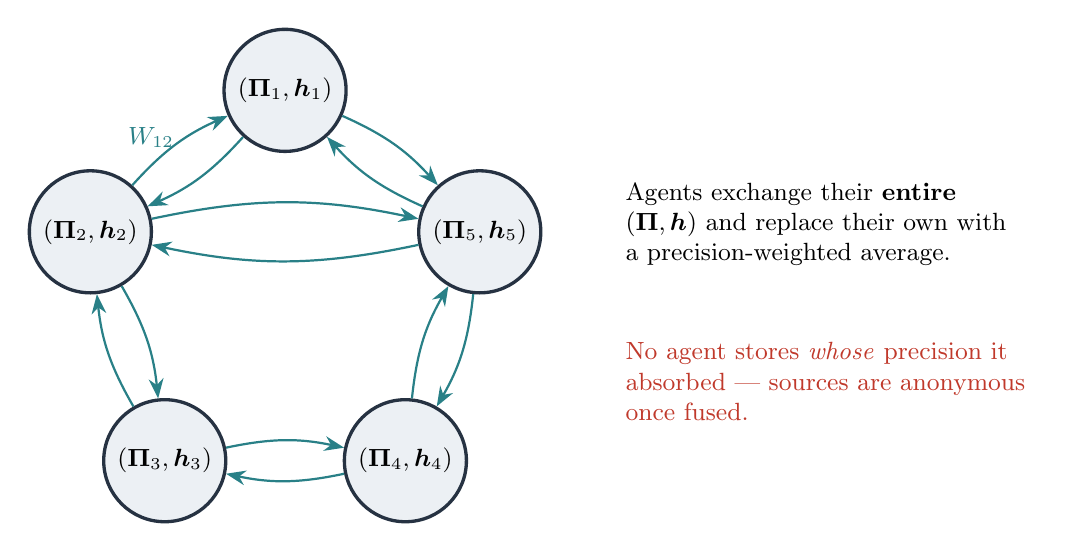
\begin{tikzpicture}[
      agent/.style={circle, draw=slate, very thick, fill=paleslate,
                    minimum size=1.55cm, font=\small},
      flow/.style={-{Stealth[length=2.5mm]}, calm, thick},
      scale=1.0]
    % ring of 5 agents
    \foreach \ang/\name in {90/1, 162/2, 234/3, 306/4, 18/5}{
      \node[agent] (a\name) at (\ang:2.6) {$(\Pii_{\name},\hh_{\name})$};
    }
    % fusion arrows (bidirectional ring + two chords)
    \foreach \u/\v in {1/2, 2/3, 3/4, 4/5, 5/1, 2/5}{
      \draw[flow] (a\u) to[bend left=12] (a\v);
      \draw[flow] (a\v) to[bend left=12] (a\u);
    }
    % one labelled weight
    \path (a1) -- (a2) node[midway, above left=2pt, calm, font=\small] {$W_{12}$};
    % annotation
    \node[align=left, anchor=west, font=\small, text width=5.4cm] at (4.2,0.9)
      {Agents exchange their \textbf{entire} $(\Pii,\hh)$ and replace their
       own with a precision-weighted average.};
    \node[align=left, anchor=west, font=\small, text=accent, text width=5.4cm] at (4.2,-1.1)
      {No agent stores \emph{whose} precision it absorbed --- sources are
       anonymous once fused.};
  \end{tikzpicture}
  \end{center}
\end{frame}

% ================================================================ 5. Theorem 1 + D2
\begin{frame}{Theorem 1: pooling is a contraction}
  \begin{block}{Pooling is a contraction\footnote[frame]{\tiny DeGroot (1974);
    contraction under fixed row-stochastic trust formalised in Catal (2024).}}
    On a connected trust graph, precision-weighted averaging contracts
    inter-agent disagreement \textbf{geometrically} toward consensus ---
    \emph{independent of content}.
  \end{block}
  \begin{center}
  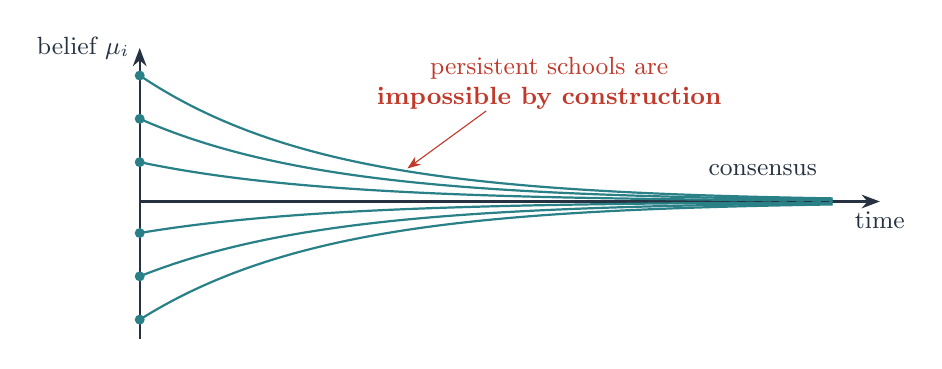
\begin{tikzpicture}[scale=1.0]
    % axes
    \draw[-{Stealth}, slate, thick] (0,-1.75) -- (0,1.95)
        node[left, font=\small] {belief $\mu_i$};
    \draw[-{Stealth}, slate, thick] (0,0) -- (9.4,0)
        node[below, font=\small] {time};
    % converging trajectories
    \foreach \y in {1.6, 1.05, 0.5, -0.4, -0.95, -1.5}{
      \draw[calm, thick, smooth, samples=60, domain=0:8.8]
        plot (\x, {\y*exp(-0.42*\x)});
      \fill[calm] (0,\y) circle (1.8pt);
    }
    % consensus line
    \draw[dashed, slate] (0,0) -- (9.0,0);
    \node[slate, font=\small, anchor=west] at (7.1,0.4) {consensus};
    % annotation
    \node[accent, font=\small, align=center] at (5.2,1.5)
      {persistent schools are\\ \textbf{impossible by construction}};
    \draw[-{Stealth}, accent] (4.4,1.15) -- (3.4,0.42);
  \end{tikzpicture}
  \end{center}
  \vspace{-0.5em}
  {\small Distrust ($W_{ij}$ small) only rescales the exponent. It buys
   \emph{time}, never a wall.}
  \vspace{0.6em}
\end{frame}

% ================================================================ 6. Theorem 2 + D3
\begin{frame}{Theorem 2: Gaussian conflict resolves by compromise}
  \begin{columns}[T]
    \column{0.52\textwidth}
      \vspace{0.4em}
      Fuse two \emph{contradictory} sources:
      \[
        \Pii = \Pii_A + \Pii_C, \quad
        \bm{\mu} = \Pii^{-1}(\Pii_A\bm{\mu}_A + \Pii_C\bm{\mu}_C)
      \]
      \begin{itemize}
        \item<1-> mean lands \textbf{between} the sources
        \item<1-> precision \textbf{adds} --- confidence \emph{grows} while
              averaging contradictions
        \item<2-> \alert{the result is a confident belief in a configuration
              neither source supports}
      \end{itemize}
      \vspace{0.3em}
      \onslide<2->{{\small Light tails cannot reject extreme sources; conflict
      is invisible to the update.\footnote[frame]{\tiny On conflict-blind
      precision pooling see O'Hagan (2012), \emph{combining probability
      distributions}.}}}
    \column{0.46\textwidth}
      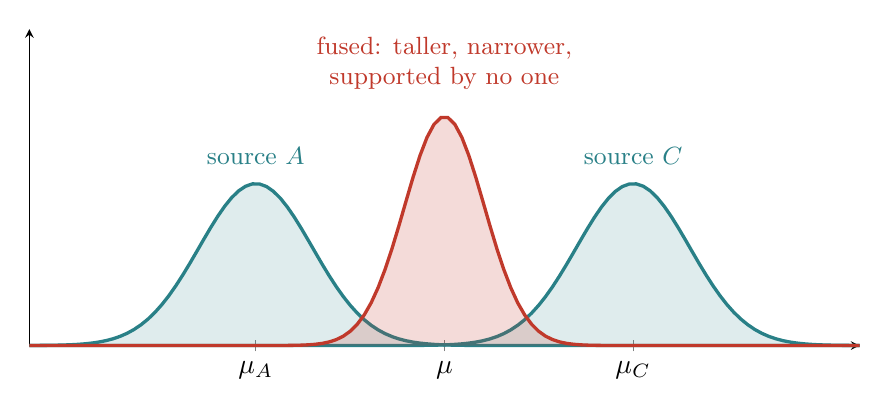
\begin{tikzpicture}
        \begin{axis}[
            width=\textwidth, height=5.6cm,
            axis lines=left, xmin=-4.4, xmax=4.4, ymin=0, ymax=1.3,
            xtick={-2,0,2}, xticklabels={$\mu_A$,$\mu$,$\mu_C$},
            ytick=\empty, samples=120, domain=-4.4:4.4,
            every axis plot/.append style={very thick},
            clip=false]
          \addplot[calm, fill=calm, fill opacity=0.15]
            {0.665*exp(-0.5*((x+2)/0.6)^2)};
          \addplot[calm, fill=calm, fill opacity=0.15]
            {0.665*exp(-0.5*((x-2)/0.6)^2)};
          \addplot[accent, fill=accent, fill opacity=0.18]
            {0.94*exp(-0.5*(x/0.424)^2)};
          \node[calm, font=\small] at (axis cs:-2,0.78) {source $A$};
          \node[calm, font=\small] at (axis cs:2,0.78) {source $C$};
          \node[accent, font=\small, align=center] at (axis cs:0,1.16)
            {fused: taller, narrower,\\ supported by no one};
        \end{axis}
      \end{tikzpicture}
  \end{columns}
\end{frame}

% ================================================================ 7. missing slot
\begin{frame}{The missing slot}
  There is \textbf{no coordinate in $(\Pii,\hh)$} whose value can mean
  ``torn between two hypotheses.''
  \vspace{0.3em}
  \begin{center}
  \small
  \renewcommand{\arraystretch}{1.25}
  \begin{tabular}{p{5.6cm}p{6.2cm}}
    \textbf{What a model of science needs} & \textbf{What the Gaussian form can store}\\
    \hline
    rival hypotheses, held simultaneously & one mean $\bm{\mu}$ \\
    represented disagreement, a ``hung jury'' & one precision $\Pii$ (always unimodal) \\
    suspended judgment under conflict & conflict $\Rightarrow$ \alert{more} confidence \\
    knowing \emph{who} disagrees, \emph{about what} & sources erased at fusion \\
  \end{tabular}
  \end{center}
  \vspace{0.3em}
  \begin{block}{}
    \small This is impoverishment \textbf{by representation}, not by
    parameters: the mean-field/Gaussian choice pulls every tension to the
    mean \emph{before} dynamics can act on it.
  \end{block}
\end{frame}

% ================================================================ 8. corollaries
\begin{frame}{What this does to a model of science}
  \begin{columns}[T]
    \column{0.52\textwidth}
      Corollaries of the two theorems:
      \begin{itemize}
        \item \textbf{The lone discoverer is averaged away.} A commitment held
          by one agent is diluted $1/N$ per fusion round --- discovery cannot
          survive its own community.
        \item \textbf{No denial, no crisis.} Anomalies just shift the mean
          smoothly; there is no regime where evidence is resisted and then
          breaks through.
        \item \textbf{Contact is always fatal to the minority.} Lock-in
          survives only by \emph{isolation}; any nonzero coupling converts the
          smaller camp.
      \end{itemize}
    \column{0.46\textwidth}
      \begin{center}
        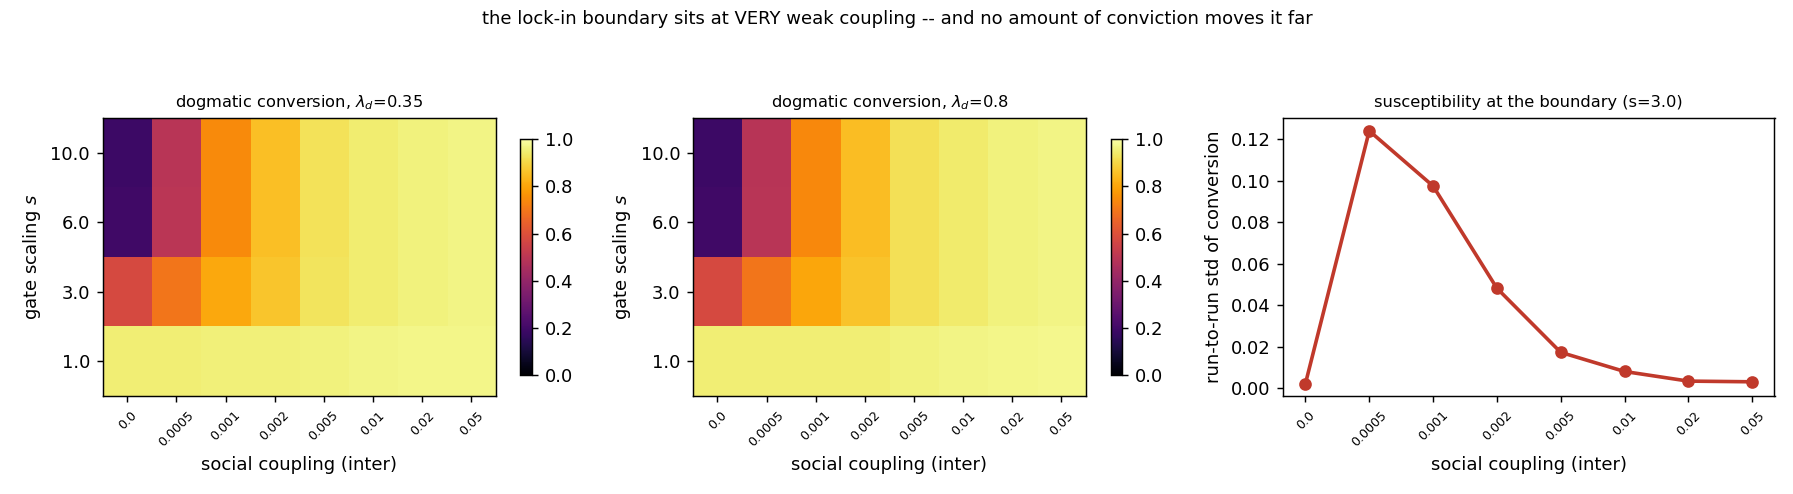
\includegraphics[width=\textwidth]{fig_kuhn_lockin_boundary.png}\\
        {\footnotesize Lock-in boundary: the dogmatic camp persists only in the
         isolated corner; faint contact collapses it.}
      \end{center}
  \end{columns}
\end{frame}

% ================================================================ 9. empirics
\begin{frame}{The simulations do exactly what the theorems say}
  \begin{columns}[T]
    \column{0.5\textwidth}
      \begin{center}
        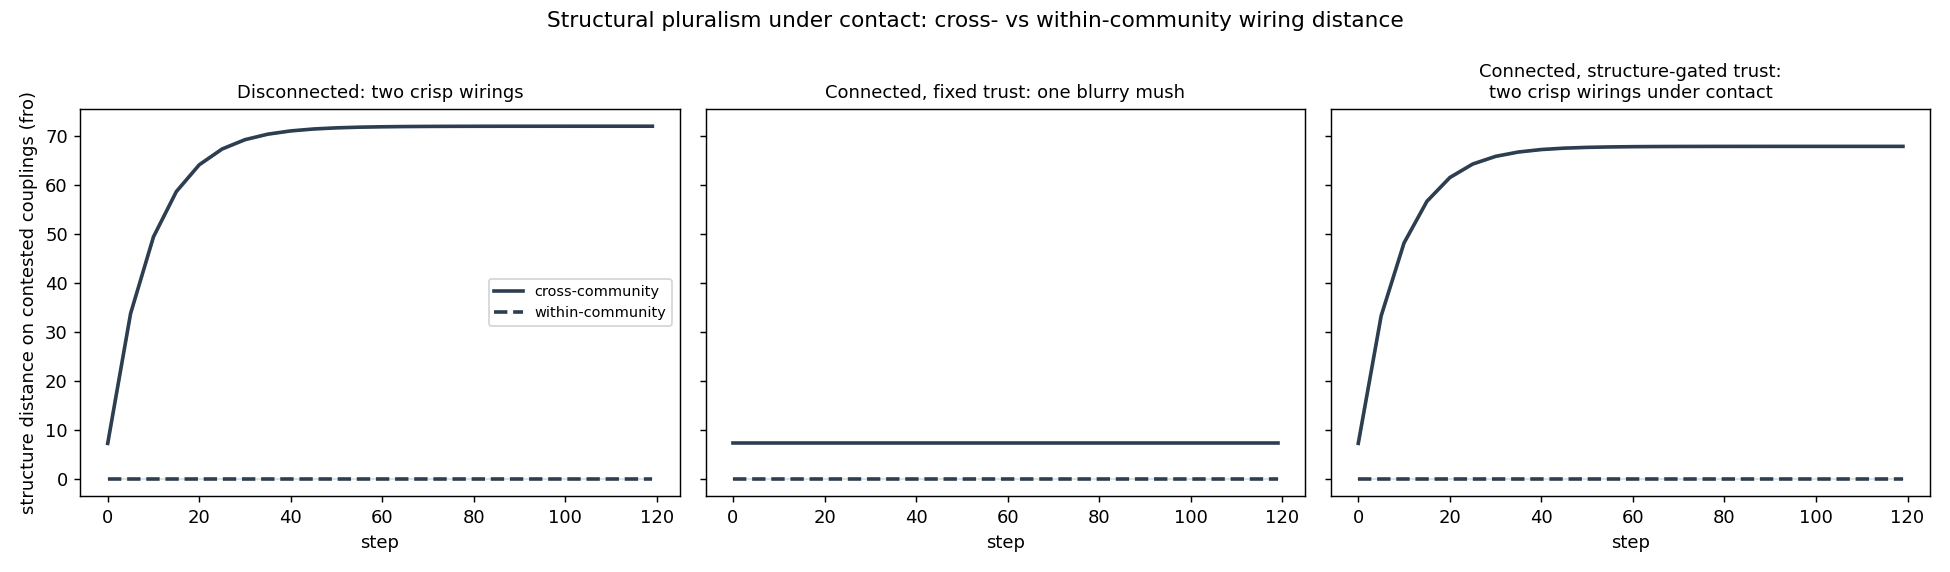
\includegraphics[width=\textwidth]{fig_divergence_traces.png}\\
        {\footnotesize Inter-camp distance $D(t)$, log scale: under fixed
         trust (baseline), divergence decays \textbf{exponentially} ---
         the contraction, measured.}
      \end{center}
    \column{0.5\textwidth}
      \begin{center}
        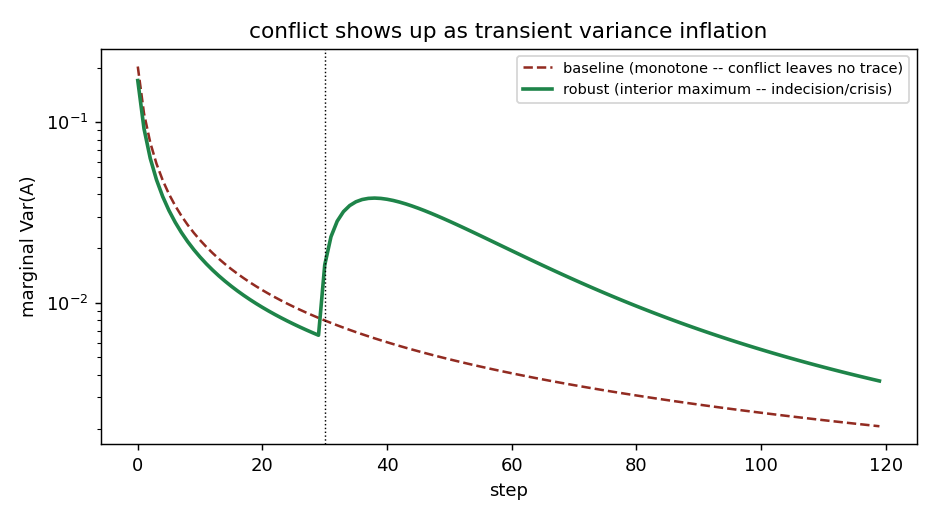
\includegraphics[width=\textwidth]{fig_abc_variance.png}\\
        {\footnotesize Conflicting sources: baseline fusion averages them with
         opposite sign and \emph{gains} confidence --- Theorem 2, measured.}
      \end{center}
  \end{columns}
  \vspace{0.4em}
  \begin{center}
    \small No parameter setting escapes this. The null result is the
    representation speaking.
  \end{center}
\end{frame}

% ================================================================ 10. D4 two nets
\begin{frame}{The capability that is missing: holding two nets at once}
  \begin{center}
  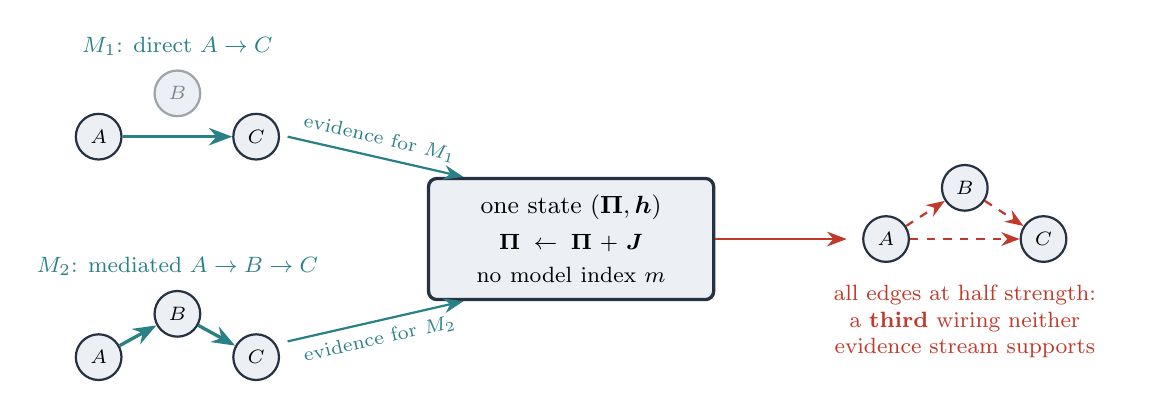
\begin{tikzpicture}[
      vert/.style={circle, draw=slate, thick, fill=paleslate,
                   minimum size=0.58cm, inner sep=1pt, font=\scriptsize},
      ghost/.style={circle, draw=slate!45, thick, fill=paleslate,
                    minimum size=0.58cm, inner sep=1pt,
                    font=\scriptsize, text=slate!60},
      state/.style={rounded corners=3pt, draw=slate, very thick,
                    fill=paleslate, font=\small, align=center, inner sep=6pt},
      flow/.style={-{Stealth[length=2.5mm]}, calm, thick},
      lbl/.style={font=\footnotesize, calm, align=center}]
    % ----- rival wiring M1: direct A->C
    \begin{scope}[xshift=-5.0cm, yshift=1.25cm]
      \node[vert] (A1) at (-1.0,-0.1) {$A$};
      \node[ghost] (B1) at ( 0.0, 0.45) {$B$};
      \node[vert] (C1) at ( 1.0,-0.1) {$C$};
      \draw[-{Stealth}, calm, very thick] (A1) -- (C1);
      \node[lbl] at (0,1.05) {$M_1$: direct $A \to C$};
    \end{scope}
    % ----- rival wiring M2: mediated A->B->C
    \begin{scope}[xshift=-5.0cm, yshift=-1.55cm]
      \node[vert] (A2) at (-1.0,-0.1) {$A$};
      \node[vert] (B2) at ( 0.0, 0.45) {$B$};
      \node[vert] (C2) at ( 1.0,-0.1) {$C$};
      \draw[-{Stealth}, calm, very thick] (A2) -- (B2);
      \draw[-{Stealth}, calm, very thick] (B2) -- (C2);
      \node[lbl] at (0,1.05) {$M_2$: mediated $A \to B \to C$};
    \end{scope}
    % ----- single state in the middle
    \node[state, text width=3.2cm] (st) at (0,-0.15)
      {one state $(\Pii,\hh)$\\[2pt]
       {\footnotesize $\Pii \leftarrow \Pii + \bm{J}$}\\[1pt]
       {\footnotesize no model index $m$}};
    \draw[flow] (-3.6,1.15) -- (st.150)
      node[midway, above, sloped, font=\scriptsize, calm]
      {evidence for $M_1$};
    \draw[flow] (-3.6,-1.45) -- (st.210)
      node[midway, below, sloped, font=\scriptsize, calm]
      {evidence for $M_2$};
    % ----- blended result on the right
    \begin{scope}[xshift=5.0cm, yshift=-0.05cm]
      \node[vert] (A3) at (-1.0,-0.1) {$A$};
      \node[vert] (B3) at ( 0.0, 0.55) {$B$};
      \node[vert] (C3) at ( 1.0,-0.1) {$C$};
      \draw[-{Stealth}, accent, thick, dashed] (A3) -- (C3);
      \draw[-{Stealth}, accent, thick, dashed] (A3) -- (B3);
      \draw[-{Stealth}, accent, thick, dashed] (B3) -- (C3);
      \node[font=\footnotesize, accent, align=center, text width=3.9cm]
        at (0,-1.15)
        {all edges at half strength:\\ a \textbf{third} wiring neither\\
         evidence stream supports};
    \end{scope}
    \draw[-{Stealth[length=2.5mm]}, accent, thick] (st.east) -- (3.5,-0.15);
  \end{tikzpicture}
  \end{center}
  \vspace{0.1em}
  {\small The state is $q(\bm{\varphi})$, not $q(\bm{\varphi}, m)$. The
   evidence that \emph{discriminates} the wirings ---
   $I(o;m) = \mathrm{JSD}\big(p(o \mid M_1),\, p(o \mid M_2)\big)$ per
   observation --- has nowhere to accumulate; it is \alert{erased at deposit
   time}. The social failure (fusing two neighbours' nets) is the same
   collapse, between heads instead of within one.}
\end{frame}

% ================================================================ 11. deeper problem
\begin{frame}{This is not just our model}
  The same wall appears wherever beliefs are pooled under a Gaussian /
  mean-field form:
  \vspace{0.4em}
  \begin{itemize}
    \item \textbf{Federated inference}\footnote[frame]{\tiny Friston et al.\
      (2023), \emph{Federated inference and belief sharing}.} ---
      \emph{prescribes} precision-weighted pooling, justified by a
      common-cause assumption. Where that assumption fails (rival paradigms),
      pooling is exactly the wrong move --- and the formalism cannot express
      its failure.
    \item \textbf{Opinion dynamics} --- DeGroot-style averaging contracts
      under any fixed trust; centuries-of-disagreement requires breaking the
      averaging, not reweighting it.\footnote[frame]{\tiny DeGroot (1974);
      Catal (2024).}
    \item \textbf{Structure learning} --- Bayesian model
      comparison\footnote[frame]{\tiny Smith et al.\ (2022), structure
      learning as Bayesian model comparison; Friston et al.\ (2018), Bayesian
      model reduction.} scores rival structures, but each agent still
      \emph{owns a single posterior} --- rivals live in the analyst's ledger,
      not in any agent's head.
  \end{itemize}
  \vspace{0.4em}
  \begin{center}
    \small The shared root: the mean approximation has no slot for a
    represented rival.
  \end{center}
\end{frame}

% ================================================================ 12. the ask
\begin{frame}{What would be required}
  Structured learning over \textbf{hypothesis spaces}, not over one precision
  matrix:
  \begin{enumerate}
    \small
    \item \textbf{Multiple structural hypotheses per agent} --- a mixture or
      discrete model index $m \in \{M_1, \dots, M_K\}$ over wirings, so an
      agent can be genuinely torn: $q_i(\bm{\varphi}, m)$, not $q_i(\bm{\varphi})$.
    \item \textbf{Divergence as state} --- the difference between candidate
      nets, $D(M_1 \Vert M_2)$, carried and updated online so an agent can
      act on \emph{where} two wirings disagree. (Models of other agents'
      nets are the social special case.)
    \item \textbf{Communication of hypotheses} --- messages that transmit
      \emph{which structure} an agent entertains (wiring, $\Pii$-pattern), not
      just means and precisions to be averaged.
  \end{enumerate}
  \vspace{0.3em}
  \begin{block}{Outlook (one line)}
    \small Inferred reliability gates (Student-$t$ trust, v4) make divergence
    \emph{metastable} --- but consensus remains the only fixed point. Gates buy
    time; only represented rivals buy walls.
  \end{block}
\end{frame}

% ================================================================ 13. ladder
\begin{frame}{How much doubt does pluralism need?}
  Each rung adds model-doubt to the \emph{state}; each unlocks dynamics ---
  and every rung but the last still converges.
  \vspace{0.4em}
  \begin{center}
  \footnotesize
  \renewcommand{\arraystretch}{1.25}
  \begin{tabular}{p{2.9cm}p{3.0cm}p{3.1cm}p{3.4cm}}
    \textbf{Representation} & \textbf{Doubt in the state} &
    \textbf{Unlocks} & \textbf{Still converges because}\\
    \hline
    Gaussian $(\Pii,\hh)$ & none & nothing (null regime) & pooling is a contraction \\
    Student-$t$ gates & doubt about sources & metastable schism & gates buy time, not walls \\
    mixture $q(\bm{\varphi},m)$ & \emph{precise} doubt about models & rivalry, suspended judgment & Berk: weights concentrate on the KL-closest $m$\footnote[frame]{\tiny Berk (1966): under misspecification the posterior converges to certainty in the KL-nearest --- possibly wrong --- model.} \\
    credal set $\{q_m\}$ & \alert{Knightian} doubt & pluralism evidence need not dissolve & \alert{it doesn't --- that is the point} \\
  \end{tabular}
  \end{center}
  \vspace{0.2em}
  {\small Precise mixtures are gates by other means: more time, still no walls
   --- permanent pluralism lives on the last rung.}
\end{frame}

% ================================================================ 14. conviction vs Knight
\begin{frame}{Does conviction buy Knightian uncertainty?}
  Tilt the weights over models: $q(m) \propto p(m \mid o)\, e^{\lambda U(m)}$.
  For two rivals,
  \[
    \log\frac{q(M_1)}{q(M_2)} \;=\;
    \underbrace{\Lambda_T}_{\text{accumulated log-evidence}}
    \;+\; \underbrace{\lambda\,\Delta U}_{\text{conviction}}
  \]
  \vspace{-0.4em}
  \begin{itemize}\small
    \item \alert{The naive limit fails.} $\lambda \to \infty$ in one head
      $\Rightarrow$ certainty in $\arg\max_m U(m)$: \alert{dogmatism}, the
      opposite of held-open ambiguity.
    \item \textbf{Timescale.} Rivals survive while
      $|\Lambda_T| < \lambda\,\Delta U$, so the merge clock is
      $T^{\ast} \approx \dfrac{\lambda\,\Delta U}{I(o;m)\ \text{per obs.}}$
      --- conviction over the channel capacity for telling models apart:
      the JSD that the Gaussian erased now sets the clock.
    \item \textbf{Duality (the precise statement).} Exponential tilts are the
      single-distribution representatives of \emph{set-based} preference
      families; maxmin Knight is the \emph{pessimistic} member
      ($e^{-\theta V}$), conviction the \emph{optimistic} one
      ($e^{+\lambda U}$).\footnote[frame]{\tiny Hansen \& Sargent (2001),
      multiplier preferences; Maccheroni, Marinacci \& Rustichini (2006),
      variational preferences; Gilboa \& Schmeidler (1989), maxmin EU.}
      \alert{Self-evidencing is ambiguity with the sign flipped} --- Knight is
      conviction's mirror twin, not its limit.
  \end{itemize}
\end{frame}

% ================================================================ 15. social credal set
\begin{frame}{Where the credal set actually lives}
  \begin{center}
  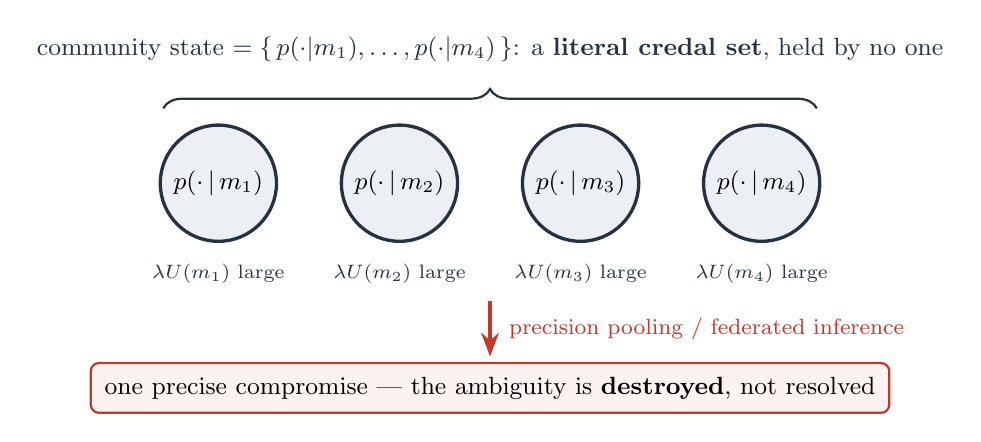
\begin{tikzpicture}[
      agent/.style={circle, draw=slate, very thick, fill=paleslate,
                    minimum size=1.05cm, font=\small, align=center},
      lbl/.style={font=\scriptsize, slate}]
    % community of convicted agents
    \foreach \x/\k in {0/1, 2.3/2, 4.6/3, 6.9/4}{
      \node[agent] (ag\k) at (\x,0) {$p(\cdot\,|\,m_{\k})$};
      \node[lbl] at (\x,-1.15) {$\lambda U(m_{\k})$ large};
    }
    \draw[decorate, decoration={brace, amplitude=7pt}, slate, thick]
      (-0.7,0.95) -- (7.6,0.95);
    \node[font=\small, slate, align=center] at (3.45,1.7)
      {community state $= \{\,p(\cdot|m_1),\dots,p(\cdot|m_4)\,\}$:
       a \textbf{literal credal set}, held by no one};
    % pooling collapse
    \draw[-{Stealth[length=3mm]}, accent, very thick]
      (3.45,-1.5) -- (3.45,-2.2)
      node[midway, right=3pt, font=\footnotesize, accent]
      {precision pooling / federated inference};
    \node[rounded corners=3pt, draw=accent, thick, fill=accent!6,
          font=\small, inner sep=5pt] at (3.45,-2.6)
      {one precise compromise --- the ambiguity is \textbf{destroyed}, not resolved};
  \end{tikzpicture}
  \end{center}
  \vspace{0.3em}
  {\small Knightian uncertainty \emph{does} drop out of strong conviction ---
   \textbf{heterogeneous} conviction, \textbf{across} heads: schools are how a
   network implements imprecise probability. Expansion (variation), reduction
   (selection), and conviction (retention) acting on $q(\bm{\varphi},m)$ keep
   the set populated; pooling collapses it.}
\end{frame}

% ================================================================ 16. summary
\begin{frame}{Summary}
  \begin{enumerate}
    \setlength{\itemsep}{0.8em}
    \item \textbf{No divergence is a theorem, not a bug.} Pooling contracts;
      Gaussian conflict resolves by confident compromise. The full model
      \emph{could not} have shown schools or schisms.
    \item \textbf{The representational slot for disagreement is missing.}
      $(\Pii,\hh)$ stores one mean and one precision; ``torn,'' ``rival,'' and
      ``who disagrees about what'' have nowhere to live.
    \item \textbf{The concrete next requirement is holding two nets at
      once.} An agent that can carry \emph{rival Bayes nets and the
      divergence between them} --- within one head or between heads ---
      so that structure-discriminating evidence accumulates instead of
      being erased at deposit time.
  \end{enumerate}
  \vspace{0.8em}
  \begin{center}
    \large Discussion: what is the minimal representation that supports a
    represented rival --- and should the credal set live in heads, or in the
    network?
  \end{center}
\end{frame}

\end{document}
